\documentclass{article}


\usepackage{arxiv}

\usepackage[utf8]{inputenc} % allow utf-8 input
\usepackage[T1]{fontenc}    % use 8-bit T1 fonts
\usepackage{hyperref}       % hyperlinks
\usepackage{url}            % simple URL typesetting
\usepackage{booktabs}       % professional-quality tables
\usepackage{amsfonts}       % blackboard math symbols
\usepackage{nicefrac}       % compact symbols for 1/2, etc.
\usepackage{microtype}      % microtypography
\usepackage{lipsum}
\usepackage{graphicx}
\usepackage{slashbox}
\usepackage{xcolor}
\usepackage{subfig}
\usepackage{todonotes}

\title{Pseudo-Boolean Encoding for Local Envy Freeness}


\author{
  Jean-Guy Mailly\\
  LIPADE -- Université de Paris\\
  Paris, France\\
  \texttt{jean-guy.mailly@u-paris.fr} \\
  %% examples of more authors
   \And
Nicolas Maudet \\
LIP6 -- Sorbonne University\\
Paris, France\\
\texttt{nicolas.maudet@lip6.fr} \\
\And
Anaelle Wilczynski\\
  Affiliation \\
  Address \\
  \texttt{anaelle.wilczynski@centralesupelec.fr} \\
  %% \And
  %% Coauthor \\
  %% Affiliation \\
  %% Address \\
  %% \texttt{email} \\
  %% \And
  %% Coauthor \\
  %% Affiliation \\
  %% Address \\
  %% \texttt{email} \\
}

\begin{document}
\maketitle

\begin{abstract}
\lipsum[1]
\end{abstract}


\section{Introduction}
See \cite{BeynierCGHLMW19}.

\section{Problem Formulation}
\begin{itemize}
	\item $O = \{o_1, \dots, o_n\}$: set of objects
	\item $N = \{1,\dots,n\}$: set of agents
	\item $\succ_i$: preferences of agent $i$ over $O$ (linear order)
	\item $G = \langle N, E\rangle$: social network (undirected graph)
\end{itemize}
{\bf Problem:} assign each agent $i$ an object $o_k$ s.t. $i$ does not prefer the object assigned to one of her neighbors, {\em i.e.} $\forall j \in N$ s.t. $\{i,j\} \in E$, $i$ does not prefers $o_l$ to $o_k$, where $o_l$ is the object assigned to $j$.

\section{Pseudo-Boolean Encoding for the Decision Problem}
\subsection{First Step: SAT Encoding}
Boolean variables:
\begin{itemize}
	\item $\forall i \in N, o_k, o_l \in O$, $pref_i^{o_k,o_l} = \top$ iff $o_k \succ_i o_l$,
	\item $\forall i \in N, o \in O$, $alloc_{i,o} = \top$ iff $o$ is allocated to $i$.
\end{itemize}

Model the allocation:
\[
\phi_{alloc} = \bigwedge_{i \in N} (\bigoplus_{o \in O} alloc_{i,o}) \wedge \bigwedge_{o \in O} (\bigoplus_{i \in N} alloc_{i,o})
\]

Model Local Envy-freeness:
\[
\phi_{lef} = \bigwedge_{\{i,j\} \in E} (\bigwedge_{o_k,o_l \in O} (alloc_{i,o_k} \wedge alloc_{j,o_l}) \rightarrow pref_i^{o_k,o_l}) \equiv \bigwedge_{\{i,j\} \in E} (\bigwedge_{o_k,o_l \in O} \neg alloc_{i,o_k} \vee \neg alloc_{j,o_l} \vee pref_i^{o_k,o_l})
\]

\subsection{Second Step: PB Encoding}
XOR are easy to encode as Pseudo-Boolean constraints. $\phi_{alloc}$ is replaced by the set of PB constraints:
\begin{description}
	\item[($PB_{alloc}^{i}$)] $\sum_{o \in O} alloc_{i,o} = 1$
	\item[($PB_{alloc}^{o}$)] $\sum_{i \in N} alloc_{i,o} = 1$
\end{description}

Clauses can be easily encoded as PB constraints as well. So $\phi_{lef}$ is replaced by the set of PB constraints:
\begin{description}
	\item[$(PB_{lef}^{i,j,o_k,o_l})$] $\neg alloc_{i,o_k} + \neg alloc_{j,o_l} + pref_i^{o_k,o_l} \geq 1$
\end{description}
where $\{i,j\} \in E$.

\section{Experimental Evaluation for DEC-LEF}\label{section:expe-dec-lef}
\subsection{Implementation and Experimental Environment}
\begin{itemize}
	\item Sat4j \cite{BerreP10} used for solving the PB instance
	\item Python script used for reading the allocation instance (social network $+$ preferences), providing the PB encoding, and parsing the output of Sat4j
	\item Experimental environment: macOS 11.5, M1 SoC (3.2GHz), 8Go RAM
\end{itemize}

\subsection{Benchmark Selection}
We have used NetworkX\footnote{See \url{https://networkx.org}.} for generating social networks following various generation patterns. For each social network with $n$ agents, we generate random preferences over $n$ objects.

\paragraph{Erd\"os-R\'enyi} For each probability $p \in \{0, 0.1, 0.3, 0.5, 0.7, 0.9, 1\}$, and each size $n \in \{10,20,30,40,50\}$, we have generated $10$ social networks with $n$ agents, and a probability $p$ that two given agents know each other.

\paragraph{Path} For each size $n \in \{10,20,30,40,50\}$, we have generated the path social network made of $n$ agents, and $10$ different (random) preferences distributions.

\paragraph{Barab\'asi-Albert} For each attachment value $m \in \{1,2,3,4,5\}$, and each size $n \in \{10,20,30,40,50\}$, we have generated $10$ social networks with $n$ agents, where each new node is connected to $m$ agents.

\paragraph{Watts-Strogatz} For each attachment value $m \in \{2,4,6,8\}$, each probability of rewiring $p \in \{0.1, 0.3, 0.5, 0.7, 0.9\}$, and each size $n \in \{10,20,30,40,50\}$, we have generated $10$ social networks with $n$ agents, an attachment $m$, and a probability $p$.

\subsection{Results}
For each category of social networks in our experiments, we describe the results regarding the runtime and the number of (non-)LEF instances, depending on the values of the various parameters. All the runtimes given are the average over the $10$ instances in each category of social networks.

\paragraph{Erd\"os-R\'enyi} Figure~\ref{fig:runtime-erdos-renyi} shows the runtime for solving DEC-LEF w.r.t. the various values of  $p$ and $n$. The impact of $p$ on the runtime is not easy to assess. Indeed, hardest instances are the ones with the lowest probability ($p = 0.0, 0.1$), {\em i.e.} the least dense social networks. On the opposite, the easiest instances are the ones with $p=0.5$, which seems to indicate that the solver performs better when the density of the social network is neither too high nor too low. 

\begin{figure}[htb]
\centering
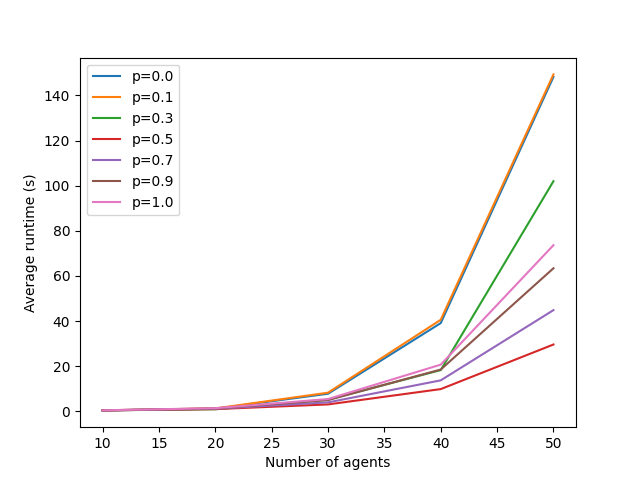
\includegraphics[width=0.45\linewidth]{results-runtime-ER.png}
\caption{Average Runtime for DEC-LEF on Erd\"os-R\'enyi Social Networks for $n \in \{10,20,30,40,50\}$\label{fig:runtime-erdos-renyi}}
\end{figure}

Table~\ref{tab:non-lef-erdos-renyi} shows the number of non-LEF instances for the same categories of instances. We observe that $p$ has an impact on the local envy-freeness, since the number of non-LEF instances increases when the probability does so. More specifically, when $p \geq 5$, all the instances but one are non-LEF. On the contrary, all the instances are LEF when $p \leq 0.1$. Only in the case $p=0.3$ there is some variability of the number of non-LEF instances. Notice that we do not observe a direct correlation between $n$ and the number of non-LEF instances.

\begin{table}[htb]
\centering
\begin{tabular}{|c|c|c|c|c|c|c|c|}
	\hline
	\backslashbox{$n$}{$p$} & $0$ & $0.1$ & $0.3$ & $0.5$ & $0.7$ & $0.9$ & $1$ \\ \hline
	$10$ & $0$ & $0$ & $2$ & $9$ & $10$ & $10$ & $10$ \\
	$20$ & $0$ & $0$ & $9$ & $10$ & $10$ & $10$ & $10$ \\
	$30$ & $0$ & $0$ & $6$ & $10$ & $10$ & $10$ & $10$ \\
	$40$ & $0$ & $0$ & $7$ & $10$ & $10$ & $10$ & $10$ \\
	$50$ & $0$ & $0$ & $4$ & $10$ & $10$ & $10$ & $10$ \\
	\hline
\end{tabular}
\caption{Number of non-LEF instance on Erd\"os-R\'enyi Social Networks for $n \in \{10,20,30,40,50\}$\label{tab:non-lef-erdos-renyi}}
\end{table}

\paragraph{Path} The runtime for solving DEC-LEF on the path social networks are shown at Figure~\ref{fig:runtime-path}. For this type of networks, all the instances used in our experiments are LEF. We observe that the impact of the network size on the runtime is similar for this type of graphs to the impact for Erd\"os-R\'enyi graphs with $p = 0.0, 0.1$. Similar observation can be made with the following categories of networks.

\begin{figure}[htb]
\centering
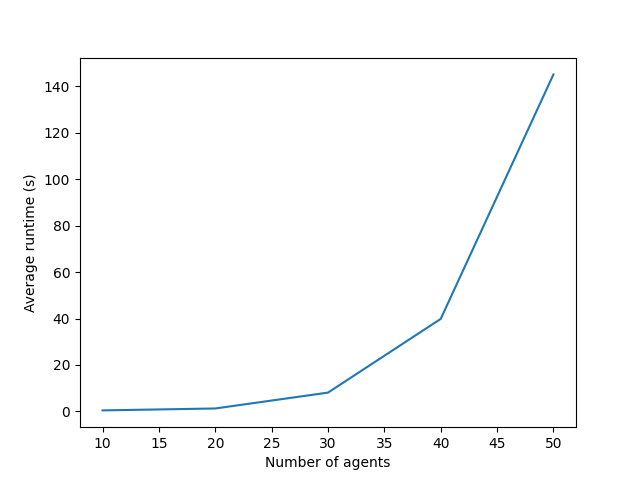
\includegraphics[width=0.45\linewidth]{results-runtime-path.png}
\caption{Average Runtime for DEC-LEF on Path Social Networks for $n \in \{10,20,30,40,50\}$\label{fig:runtime-path}}
\end{figure}

\paragraph{Barab\'asi-Albert} Figure~\ref{fig:runtime-barabasi-albert} shows the runtime for solving DEC-LEF w.r.t. the various values of  $m$ and $n$. Table~\ref{tab:non-lef-barabasi-albert} shows the number of non-LEF instances for the same categories. The value of $m$ has no significant impact on the runtime, but it increases the number of non-LEF instances. Observe that, contrary to the case of Erd\"os-R\'enyi networks, here the value of $n$ has a clear impact on the number of non-LEF instances: the higher is $n$, the lower is the number of non-LEF instances, with all the instances being LEF when $n=50$.

\begin{figure}[htb]
\centering
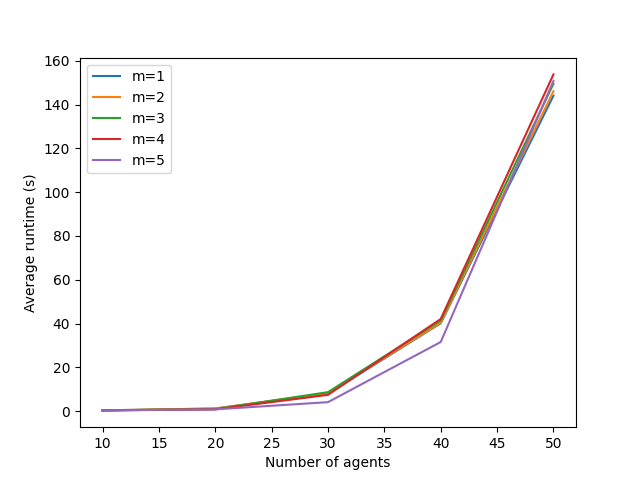
\includegraphics[width=0.45\linewidth]{results-runtime-BA.png}
\caption{Average Runtime for DEC-LEF on Barab\'asi-Albert Social Networks for $n \in \{10,20,30,40,50\}$\label{fig:runtime-barabasi-albert}}
\end{figure}

\begin{table}[htb]
\centering
\begin{tabular}{|c|c|c|c|c|c|}
	\hline
	\backslashbox{$n$}{$m$} & $1$ & $2$ & $3$ & $4$ & $5$ \\ \hline
	$10$ & $0$ & $8$ & $10$ & $9$ & $10$ \\
	$20$ & $0$ & $1$ & $7$ & $9$ & $10$ \\
	$30$ & $0$ & $0$ & $0$ & $2$ & $7$ \\
	$40$ & $0$ & $0$ & $0$ & $0$ & $3$ \\
	$50$ & $0$ & $0$ & $0$ & $0$ & $0$ \\
	\hline
\end{tabular}
\caption{Number of non-LEF instance on Barab\'asi-Albert Social Networks for $n \in \{10,20,30,40,50\}$\label{tab:non-lef-barabasi-albert}}
\end{table}

\paragraph{Watts-Strogatz} Runtimes for Watts-Strogatz instances are shown at Figure~\ref{fig:runtime-watts-strogatz}, with each subfigure corresponding to a different value of  $m $. The general observation is the same as for previous categories: neither $m$ nor $p$ has a significant impact on the runtime (at the exception of $m=4$ and $p=0.7$, where one instance was solved in more than $2300$ seconds, instead of $145$ seconds for other instances of the same size, hence the higher average runtime).

\begin{figure}[htb]
\centering
\subfloat[$m=2$\label{fig:runtime-watts-strogatz-2}]{
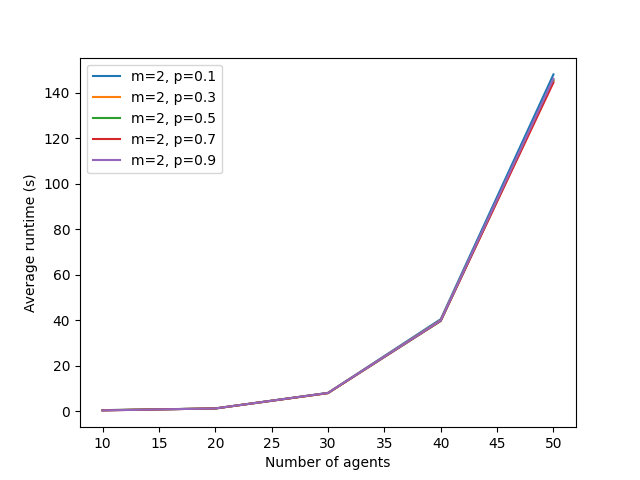
\includegraphics[width=0.45\linewidth]{results-runtime-WS-2.png}
}
\subfloat[$m=4$\label{fig:runtime-watts-strogatz-4}]{
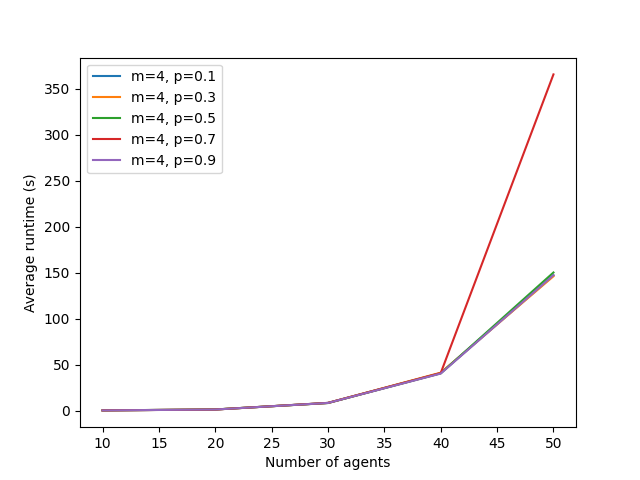
\includegraphics[width=0.45\linewidth]{results-runtime-WS-4.png}
}

\subfloat[$m=6$\label{fig:runtime-watts-strogatz-6}]{
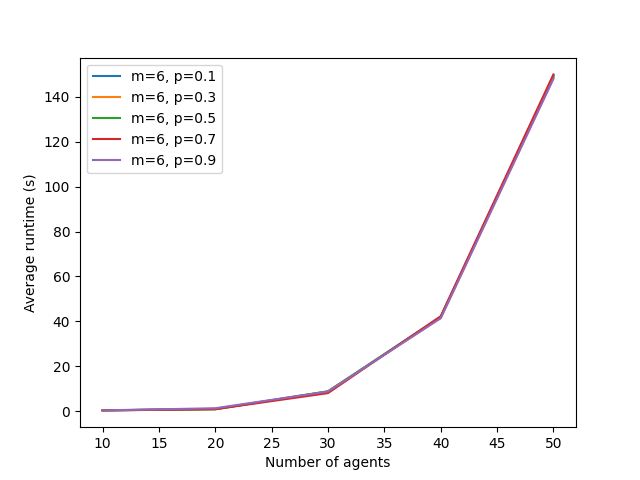
\includegraphics[width=0.45\linewidth]{results-runtime-WS-6.png}
}
\subfloat[$m=8$\label{fig:runtime-watts-strogatz-8}]{
 \missingfigure[figwidth=0.45\linewidth,figheight=4.9cm]{Placeholder}
}
\caption{Average Runtime for DEC-LEF on Watts-Strogatz Social Networks and $n \in \{10,20,30,40,50\}$\label{fig:runtime-watts-strogatz}}
\end{figure}

\section{Pseudo-Boolean Encoding for the Optimization Problem}
\begin{itemize}
	\item $O = \{o_1, \dots, o_n\}$: set of objects
	\item $N = \{1,\dots,n\}$: set of agents
	\item $\succ_i$: preferences of agent $i$ over $O$ (linear order)
	\item $G = \langle N, E\rangle$: social network (undirected graph)
\end{itemize}
{\bf Problem:} assign each agent $i$ an object $o_k$ s.t. the number of LEF agents is maximal.
%$i$ does not prefer the object assigned to one of her neighbors, {\em i.e.} $\forall j \in N$ s.t. $\{i,j\} \in E$, $i$ does not prefers $o_l$ to $o_k$, where $o_l$ is the object assigned to $j$.

The encoding is almost the same as in the previous case, except that the constraint
\begin{description}
	\item[$(PB_{lef}^{i,j,o_k,o_l})$] $\neg alloc_{i,o_k} + \neg alloc_{j,o_l} + pref_i^{o_k,o_l} \geq 1$
\end{description}
%where $\{i,j\} \in E$.
is replaced by
\begin{description}
	\item[$(PB_{lef}^{i,j,o_k,o_l})$] $\neg alloc_{i,o_k} + \neg alloc_{j,o_l} + pref_i^{o_k,o_l} + non\_lef_i \geq 1$
\end{description}
where $non\_lef_i$ is a newly introduced Boolean variable which is true iff the agent $i$ is not LEF: the variable is assigned $\top$ in order to satisfy the constraint in the case where the rest of the constraint is not satisfy. Then, an objective function is added:
\begin{description}
	\item[(Obj)] \verb+minimize+ $\sum_{i \in N} non\_lef_i$
\end{description}


\section{Ideas}
Easy ones:
\begin{itemize}
	\item Preferential attachment for generating the graphs
	\item Study the ratio of yes/no instances
	\item Study the cost of the optimal solutions
	\item Can we complete a partial allocation into a LEF allocation?
	\item Can we obtain a LEF allocation with a given set of forbidden pairs agent/object?
\end{itemize}

Harder ones:
\begin{itemize}
	\item Constraint on the preferences (single peaked,...)
	\item MUS of the UNSAT instances (explicability of negative results)
	\item $k$-local envy freeness (look at the $k$ neighbors)
	\item Use the non-envy graph
	\item Sequence of swaps (from a given allocation, can we reach a LEF allocation?)
	\item Variant: each agent can have several objects, each object has an utility, and she is envy-free if the sum of the utilities is greater or equal to the sum of the utility of her neighbors' bundle
	\[
	\sum_{o_k} alloc_{i,o_k} \times u_{i,o_k} \geq \sum_{o_k} alloc_{j,o_k} \times u_{i,o_k}
	\]
\end{itemize}

\appendix

\section{Preliminary Experimental Evaluation for DEC-LEF}\label{section:prelim-expe-dec-lef}
\subsection{Implementation and Experimental Environment}
\begin{itemize}
	\item Sat4j \cite{BerreP10} used for solving the PB instance
	\item Python script used for reading the allocation instance (social network $+$ preferences), providing the PB encoding, and parsing the output of Sat4j
	\item Experimental environment: macOS 11.5, M1 SoC (3.2GHz), 8Go RAM
\end{itemize}

\subsection{Random Social Network}
\subsubsection{Protocol}
\begin{itemize}
	\item Social networks: Erdos-Renyi graphs with probability $p \in \{0.3, 0.5, 0.7\}$
	\item For each $p$ and each size $n \in \{10,20,30,40,50\}$, $10$ instances are generated
	\item The preferences of each agent are a random shuffle of the list of objects $[o_1,\dots,o_n]$
\end{itemize}

\subsubsection{Results}
\begin{figure}[htb]
\centering
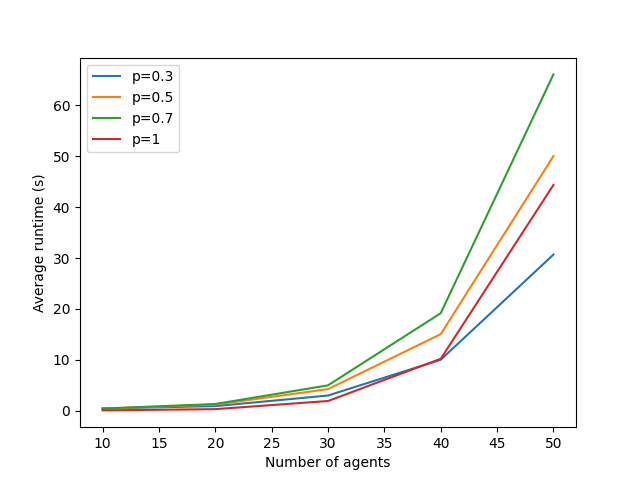
\includegraphics[width=0.5\linewidth]{prelim-random-results.png}
\caption{Preliminary Results for DEC-LEF: Average Runtime on Random Graphs for $n \in \{10,20,30,40,50\}$}
\end{figure}

\subsection{Line Social Network}
\begin{itemize}
	\item Line made of $n \in \{10, 20, 30, 40, 50\}$ agents
	\item The preferences of each agent are a random shuffle of the list of objects $[o_1,\dots,o_n]$
\end{itemize}

\subsubsection{Results}
\begin{figure}[htb]
\centering
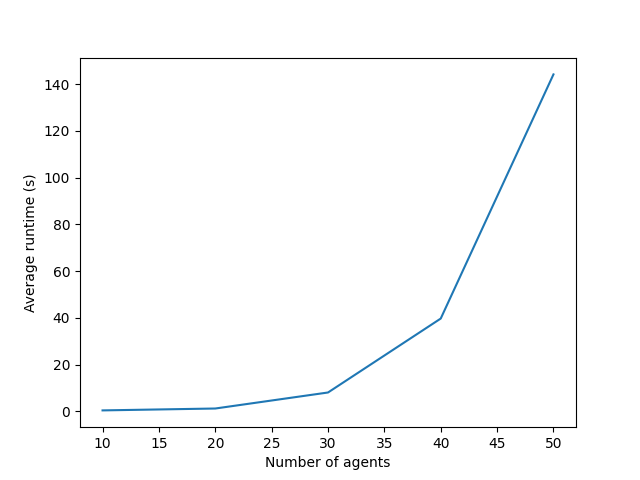
\includegraphics[width=0.5\linewidth]{prelim-line-results.png}
\caption{Preliminary Results for DEC-LEF: Average Runtime on Lines for $n \in \{10,20,30,40,50\}$}
\end{figure}

\section{Preliminary Experimental Evaluation for MAX-LEF}
\subsection{Implementation and Protocol}
Same as Section~\ref{section:expe-dec-lef}.

\subsection{Results}
\begin{figure}[htb]
\centering
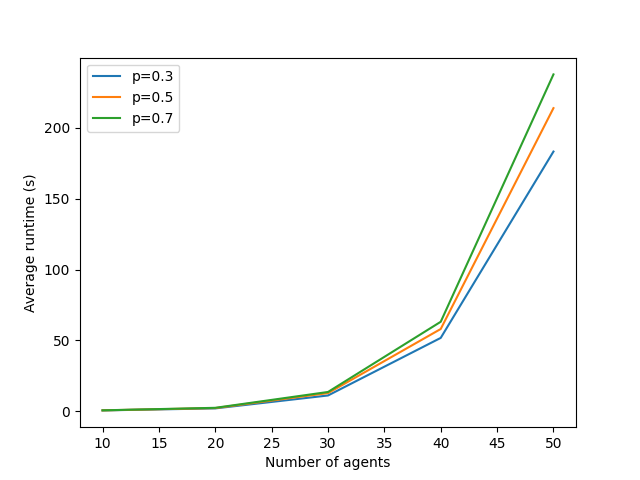
\includegraphics[width=0.5\linewidth]{prelim-results-optim.png}
\caption{Preliminary Results for MAX-LEF: Average Runtime for $n \in \{10,20,30,40,50\}$}
\end{figure}

\section{Related Work}
To read and discuss:
\begin{itemize}
	\item \cite{Bredereck0N18}: directed graph. No experiments.
	\item \cite{GanSV19}: no social network, there are $m$ houses for $n$ agents. No experiments.
	\item \cite{EibenGHO20} studies parameterized complexity. No experiments.
\end{itemize}

\bibliographystyle{unsrt}  
\bibliography{references} 
\end{document}
